%%%%%%%%%%%%%%%%%%%%%%%%%%%%%%%%%%%%%%%%%%%%%%%%%%%%%%%%%%%%%%%%%%%%%%%%%%%%%
%%%%%%%%%%%%%%%%%%%%%%%%%%%%%%%%%%%%%%%%%%%%%%%%%%%%%%%%%%%%%%%%%%%%%%%%%%%%%
\section{3D parametric cubic spline }
A 3D parametric cubic spline is a parametric function defined piecewise by parametric polynomials in $\mathbb{R}^{3}$ space.
The Fig. \ref{fig:3DSplinePoly} shows the polynomials $\mathbf{p}^{(n)}(t)$ with parameter $t$ 
close to the n-th position.
\begin{figure}[H]
    \centering
    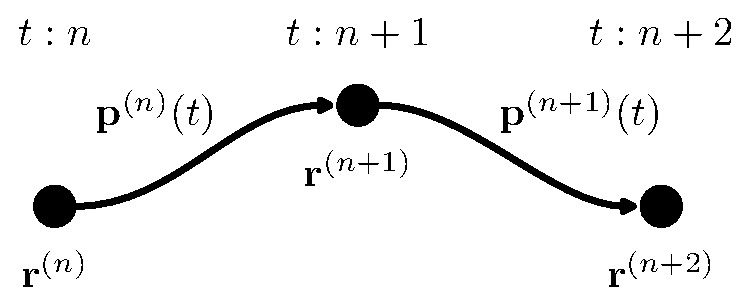
\includegraphics[width=0.35\textwidth]{boveda/Diagrama1.eps}
    \caption{Polynomials in the n-th position of cubic spline}
    \label{fig:3DSplinePoly}
\end{figure}

Given a set of $N$ points $\mathbf{r}^{(n)}\in\mathbb{R}^{3}$, $\forall$ $0\leq n \leq N-1$, 
we can generate a cubic spline with $N-2$ polynomials $\mathbf{p}^{(n)}(t)$, $\forall$ $0\leq n \leq N-2$, 
according the Fig. \ref{fig:3DSplinePoly}.
So that, it is fulfilled that 

\begin{equation}
\mathbf{p}^{(n)}(t)=
\begin{bmatrix}
p_{x}^{(n)}(t) & p_{y}^{(n)}(t) & p_{z}^{(n)}(t),
\end{bmatrix}^{T}
\end{equation}
where
\begin{equation}
p_{x}^{(n)}(t)=a_{x}^{(n)}+b_{x}^{(n)}(t-n)+c_{x}^{(n)}(t-n)^{2}+d_{x}^{(n)}(t-n)^{3},
\end{equation}
\begin{equation}
p_{y}^{(n)}(t)=a_{y}^{(n)}+b_{y}^{(n)}(t-n)+c_{y}^{(n)}(t-n)^{2}+d_{y}^{(n)}(t-n)^{3},
\end{equation}
\begin{equation}
p_{z}^{(n)}(t)=a_{z}^{(n)}+b_{z}^{(n)}(t-n)+c_{z}^{(n)}(t-n)^{2}+d_{z}^{(n)}(t-n)^{3}.
\end{equation}

%%%%%%%%%%%%%%%%%%%%%%%%%%%%%%%%%%%%%%%%%%%%%%%%%%%%%%%%%%%%%%%%%%%%%%%%%%%%%
\subsection{Matricial form of polynomials $\mathbf{p}^{(n)}(t)$}
For all values $0\leq n \leq N-2$, we know that
\begin{equation}
\mathbf{w}^{(n)}=
\left[
\begin{array}{cccc:cccc:cccc}
a_{x}^{(n)} & b_{x}^{(n)} & c_{x}^{(n)} & d_{x}^{(n)} & 
a_{y}^{(n)} & b_{y}^{(n)} & c_{y}^{(n)} & d_{y}^{(n)} & 
a_{z}^{(n)} & b_{z}^{(n)} & c_{z}^{(n)} & d_{z}^{(n)}
\end{array}
\right]^{T},
\end{equation}
\small
\begin{equation}\label{eq:Ant}
\mathbf{A}^{(n)}(t)=
\left[
\begin{array}{cccc:cccc:cccc}
1 & (t-n) & (t-n)^{2} & (t-n)^{3} &
0 & 0 & 0 & 0 &
0 & 0 & 0 & 0 \\
0 & 0 & 0 & 0 &
1 & (t-n) & (t-n)^{2} & (t-n)^{3} &
0 & 0 & 0 & 0 \\
0 & 0 & 0 & 0 &
0 & 0 & 0 & 0 &
1 & (t-n) & (t-n)^{2} & (t-n)^{3} 
\end{array}
\right],
\end{equation}
\normalsize

\begin{equation}\label{eq:primeder0}
\mathbf{p}^{(n)}(t)=
\mathbf{A}^{(n)}(t) \mathbf{w}^{(n)}.
\end{equation}

Additionally, we can define

\begin{equation}
\mathbf{w}
\equiv
\begin{bmatrix}
\mathbf{w}^{(0)}\\
\mathbf{w}^{(1)}\\
%\mathbf{w}^{(2)}\\
\vdots\\
\mathbf{w}^{(N-2)}\\
\end{bmatrix}
\in \mathbb{R}^{12(N-1)}
\end{equation}

%%%%%%%%%%%%%%%%%%%%%%%%%%%%%%%%%%%%%%%%%%%%%%%%%%%%%%%%%%%%%%%%%%%%%%%%%%%%%
\subsection{Additional useful derivation of $\mathbf{p}^{(n)}(t)$}

\small
\begin{equation}\label{eq:primeder1}
\frac{\partial \mathbf{A}^{(n)}(t)}{\partial t}=
\left[
\begin{array}{cccc:cccc:cccc}
0 & 1 & 2(t-n) & 3(t-n)^{2} &
0 & 0 & 0 & 0 &
0 & 0 & 0 & 0 \\
0 & 0 & 0 & 0 &
0 & 1 & 2(t-n) & 3(t-n)^{2} &
0 & 0 & 0 & 0 \\
0 & 0 & 0 & 0 &
0 & 0 & 0 & 0 &
0 & 1 & 2(t-n) & 3(t-n)^{2} 
\end{array}
\right],
\end{equation}
\normalsize

\small
\begin{equation}\label{eq:primeder2}
\frac{\partial^{2} \mathbf{A}^{(n)}(t)}{\partial t^{2}}=
\left[
\begin{array}{cccc:cccc:cccc}
0 & 0 & 2 & 6(t-n) &
0 & 0 & 0 & 0 &
0 & 0 & 0 & 0 \\
0 & 0 & 0 & 0 &
0 & 0 & 2 & 6(t-n) &
0 & 0 & 0 & 0 \\
0 & 0 & 0 & 0 &
0 & 0 & 0 & 0 &
0 & 0 & 2 & 6(t-n) 
\end{array}
\right].
\end{equation}
\normalsize

 If we define 
 $\frac{\partial \mathbf{A}^{(n)}(t)}{\partial t} \equiv D_{t}\mathbf{A}^{(n)}(t)$
 and
 $\frac{\partial^{2} \mathbf{A}^{(n)}(t)}{\partial t^{2}} \equiv D_{t}^{2}\mathbf{A}^{(n)}(t)$, 
 then
 
\begin{equation}\label{eq:primeder3}
\frac{\partial \mathbf{p}^{(n)}(t)}{\partial t}
=
D_{t}\mathbf{A}^{(n)}(t) \mathbf{w}^{(n)} 
\qquad
\wedge
\qquad
\frac{\partial^{2} \mathbf{p}^{(n)}(t)}{\partial t^{2}}
=
D_{t}^{2}\mathbf{A}^{(n)}(t) \mathbf{w}^{(n)}.
\end{equation}

%%%%%%%%%%%%%%%%%%%%%%%%%%%%%%%%%%%%%%%%%%%%%%%%%%%%%%%%%%%%%%%%%%%%%%%%%%%%%
%%%%%%%%%%%%%%%%%%%%%%%%%%%%%%%%%%%%%%%%%%%%%%%%%%%%%%%%%%%%%%%%%%%%%%%%%%%%%
\section{Boundary conditions in 3D parametric cubic spline}\label{sec:boundarycubic}

%%%%%%%%%%%%%%%%%%%%%%%%%%%%%%%%%%%%%%%%%%%%%%%%%%%%%%%%%%%%%%%%%%%%%%%%%%%%%
\subsection{Conditions in points}

Following the Fig. \ref{fig:3DSplinePoly}, 
we can affirm that for $0 \leq n\leq N-2$,
so that
\begin{equation}\label{eq:condition1}
\mathbf{p}^{(n)}(n)=\mathbf{r}^{(n)}
\in \mathbb{R}^{3},
\end{equation}

\begin{equation}\label{eq:condition2}
\mathbf{p}^{(N-2)}(N-1)=\mathbf{r}^{(N-1)}
\in \mathbb{R}^{3},
\end{equation}

\subsubsection{Matricial form of the conditions in points}
Using 
the Eq. \ref{eq:primeder0} in 
the Eqs. \ref{eq:condition1} and \ref{eq:condition2},
we obtain for $0 \leq n\leq N-2$

\begin{equation}\label{eq:pointcond1}
\mathbf{A}^{(n)}(n) \mathbf{w}^{(n)}=\mathbf{r}^{(n)}
\in \mathbb{R}^{3},
\end{equation}

\begin{equation}\label{eq:pointcond2}
\mathbf{A}^{(N-2)}(N-1) \mathbf{w}^{(N-2)}=\mathbf{r}^{(N-1)}
\in \mathbb{R}^{3},
\end{equation}


where, using the Eq. \ref{eq:Ant}, we know that

\begin{equation}\label{eq:Q00}
\mathbf{A}^{(n)}(n+1)=
\left[
\begin{array}{cccc:cccc:cccc}
1 & 1 & 1 & 1 &
0 & 0 & 0 & 0 &
0 & 0 & 0 & 0 \\
0 & 0 & 0 & 0 &
1 & 1 & 1 & 1 &
0 & 0 & 0 & 0 \\
0 & 0 & 0 & 0 &
0 & 0 & 0 & 0 &
1 & 1 & 1 & 1 
\end{array}
\right]
\equiv \mathbf{Q}^{(0,0)}\in \mathbb{R}^{3\times 12},
\end{equation}

\begin{equation}\label{eq:Q01}
\mathbf{A}^{(n+1)}(n+1)
=
\mathbf{A}^{(n)}(n)
=
\left[
\begin{array}{cccc:cccc:cccc}
1 & 0 & 0 & 0 &
0 & 0 & 0 & 0 &
0 & 0 & 0 & 0 \\
0 & 0 & 0 & 0 &
1 & 0 & 0 & 0 &
0 & 0 & 0 & 0 \\
0 & 0 & 0 & 0 &
0 & 0 & 0 & 0 &
1 & 0 & 0 & 0 
\end{array}
\right]
\equiv \mathbf{Q}^{(0,1)}\in \mathbb{R}^{3\times 12},
\end{equation}

Thus,
using the Eqs. \ref{eq:Q00} and \ref{eq:Q01} in 
the Eqs. \ref{eq:pointcond1} and \ref{eq:pointcond2}, 
$\forall 0 \leq n\leq N-2$;
We can write the Eqs. \ref{eq:condition1} and \ref{eq:condition2} as 

\begin{equation}
\mathbf{P}
\mathbf{w}
=\mathbf{r}\in \mathbb{R}^{3N}.
\end{equation}

Where
\begin{equation}
\mathbf{P}
\equiv
\begin{bmatrix}
\mathbf{Q}^{(0,1)} & \mathbf{0}         & \hdots & \mathbf{0} & \mathbf{0}         & \mathbf{0}\\
\mathbf{0}         & \mathbf{Q}^{(0,1)} & \hdots & \mathbf{0} & \mathbf{0}         & \mathbf{0}\\
\vdots             & \vdots             & \vdots & \vdots     & \vdots             & \vdots    \\ 
\mathbf{0}         & \mathbf{0}         & \hdots & \mathbf{0} & \mathbf{Q}^{(0,1)} & \mathbf{0}\\
\mathbf{0}         & \mathbf{0}         & \hdots & \mathbf{0} & \mathbf{0}         & \mathbf{Q}^{(0,1)}\\
\mathbf{0}         & \mathbf{0}         & \hdots & \mathbf{0} & \mathbf{0}         & \mathbf{Q}^{(0,0)}
\end{bmatrix}
\in \mathbb{R}^{3N\times 12(N-1)}
\end{equation}

and

\begin{equation}
\mathbf{r}
\equiv
\begin{bmatrix}
\mathbf{r}^{(0)}\\
\mathbf{r}^{(1)}\\
%\mathbf{w}^{(2)}\\
\vdots\\
\mathbf{r}^{(N-1)}\\
\end{bmatrix}
\in \mathbb{R}^{3N}
\end{equation}


%%%%%%%%%%%%%%%%%%%%%%%%%%%%%%%%%%%%%%%%%%%%%%%%%%%%%%%%%%%%%%%%%%%%%%%%%%%%%
\subsection{Boundary conditions in internal point}
Following the Fig. \ref{fig:3DSplinePoly}, 
we can affirm that for $0 \leq n\leq N-3$,
so that
\begin{equation}\label{eq:bound1}
\mathbf{p}^{(n)}(n+1)-\mathbf{p}^{n+1}(n+1)
=
\mathbf{0}\in \mathbb{R}^{3},
\end{equation}

\begin{equation}\label{eq:bound2}
\left.\frac{\partial\mathbf{p}^{(n)}(t)}{\partial t}\right|_{t=n+1}
-
\left.\frac{\partial\mathbf{p}^{n+1}(t)}{\partial t}\right|_{t=n+1}
=\mathbf{0}\in \mathbb{R}^{3},
\end{equation}

\begin{equation}\label{eq:bound3}
\left.\frac{\partial^{2}\mathbf{p}^{(n)}(t)}{\partial t^{2}}\right|_{t=n+1}
-
\left.\frac{\partial^{2}\mathbf{p}^{n+1}(t)}{\partial t^{2}}\right|_{t=n+1}
=\mathbf{0}\in \mathbb{R}^{3}.
\end{equation}

\subsubsection{Matricial form of the boundary conditions in internal point equation's}
Using % 
the Eqs. \ref{eq:primeder0}, \ref{eq:primeder1}, \ref{eq:primeder2} and \ref{eq:primeder3} in 
the Eqs. \ref{eq:bound1}, \ref{eq:bound2} and \ref{eq:bound3},
we obtain for $0 \leq n\leq N-3$
\begin{equation}
 \mathbf{A}^{(n)}(n+1) \mathbf{w}^{(n)} - \mathbf{A}^{n+1}(n+1) \mathbf{w}^{(n+1)} 
 =
 \mathbf{0} \in \mathbb{R}^{3},
\end{equation}

\begin{equation}
D_{t}\mathbf{A}^{(n)}(n+1)
\mathbf{w}^{(n)}
-
D_{t}\mathbf{A}^{n+1}(n+1)
\mathbf{w}^{(n+1)}
=\mathbf{0}\in \mathbb{R}^{3},
\end{equation}


\begin{equation}
D_{t}^{2}\mathbf{A}^{(n)}(n+1)
\mathbf{w}^{(n)}
-
D_{t}^{2}\mathbf{A}^{n+1}(n+1)
\mathbf{w}^{(n+1)}
=\mathbf{0}\in \mathbb{R}^{3}.
\end{equation}

Grouping in a matrix

\begin{equation}
\begin{bmatrix}
\mathbf{A}^{(n)}(n+1) & -\mathbf{A}^{n+1}(n+1)\\
D_{t}\mathbf{A}^{(n)}(n+1) & -D_{t}\mathbf{A}^{n+1}(n+1)\\
D_{t}^{2}\mathbf{A}^{(n)}(n+1) & -D_{t}^{2}\mathbf{A}^{n+1}(n+1)
\end{bmatrix}
\begin{bmatrix}
\mathbf{w}^{(n)}\\
\mathbf{w}^{(n+1)}
\end{bmatrix}
=\mathbf{0}\in \mathbb{R}^{9},
\end{equation}


using the Eqs. \ref{eq:primeder1} and \ref{eq:primeder2}, 
we know that

\begin{equation}\label{eq:Q10}
D_{t} \mathbf{A}^{(n)}(n+1)
=
\left[
\begin{array}{cccc:cccc:cccc}
0 & 1 & 2 & 3 &
0 & 0 & 0 & 0 &
0 & 0 & 0 & 0 \\
0 & 0 & 0 & 0 &
0 & 1 & 2 & 3 &
0 & 0 & 0 & 0 \\
0 & 0 & 0 & 0 &
0 & 0 & 0 & 0 &
0 & 1 & 2 & 3 
\end{array}
\right]
\equiv \mathbf{Q}^{(1,0)}\in \mathbb{R}^{3\times 12},
\end{equation}

\begin{equation}\label{eq:Q11}
D_{t} \mathbf{A}^{n+1}(n+1)
=
\left[
\begin{array}{cccc:cccc:cccc}
0 & 1 & 0 & 0 &
0 & 0 & 0 & 0 &
0 & 0 & 0 & 0 \\
0 & 0 & 0 & 0 &
0 & 1 & 0 & 0 &
0 & 0 & 0 & 0 \\
0 & 0 & 0 & 0 &
0 & 0 & 0 & 0 &
0 & 1 & 0 & 0 
\end{array}
\right]
\equiv \mathbf{Q}^{(1,1)}\in \mathbb{R}^{3\times 12},
\end{equation}

\begin{equation}\label{eq:Q20}
D_{t}^{2} \mathbf{A}^{(n)}(n+1)
=
\left[
\begin{array}{cccc:cccc:cccc}
0 & 0 & 2 & 6 &
0 & 0 & 0 & 0 &
0 & 0 & 0 & 0 \\
0 & 0 & 0 & 0 &
0 & 0 & 2 & 6 &
0 & 0 & 0 & 0 \\
0 & 0 & 0 & 0 &
0 & 0 & 0 & 0 &
0 & 0 & 2 & 6 
\end{array}
\right]
\equiv \mathbf{Q}^{(2,0)}\in \mathbb{R}^{3\times 12},
\end{equation}

\begin{equation}\label{eq:Q21}
D_{t}^{2} \mathbf{A}^{n+1}(n+1)
=
\left[
\begin{array}{cccc:cccc:cccc}
0 & 0 & 2 & 0 &
0 & 0 & 0 & 0 &
0 & 0 & 0 & 0 \\
0 & 0 & 0 & 0 &
0 & 0 & 2 & 0 &
0 & 0 & 0 & 0 \\
0 & 0 & 0 & 0 &
0 & 0 & 0 & 0 &
0 & 0 & 2 & 0 
\end{array}
\right]
\equiv \mathbf{Q}^{(2,1)}\in \mathbb{R}^{3\times 12}.
\end{equation}

Thus,
using the Eqs. \ref{eq:Q00}, \ref{eq:Q01}, \ref{eq:Q10}, \ref{eq:Q11}, \ref{eq:Q20} and \ref{eq:Q21} in 
the Eqs. \ref{eq:bound1}, \ref{eq:bound2} and \ref{eq:bound3}, 
these can be rewritten for $0 \leq n\leq N-3$

\begin{equation}
\begin{bmatrix}
\mathbf{Q}^{(0,0)} & -\mathbf{Q}^{(0,1)}\\
\mathbf{Q}^{(1,0)} & -\mathbf{Q}^{(1,1)}\\
\mathbf{Q}^{(2,0)} & -\mathbf{Q}^{(2,1)}\\
\end{bmatrix}
\begin{bmatrix}
\mathbf{w}^{(n)}\\
\mathbf{w}^{(n+1)}
\end{bmatrix}
=\mathbf{0}\in \mathbb{R}^{9}
\end{equation}

Finally, 
concatenating to all values for $0 \leq n\leq N-3$
in the boundary conditions in internal point equation's, we obtain

\begin{equation}
\mathbf{Q}
\equiv
\begin{bmatrix}
\mathbf{Q}^{(0,0)} & -\mathbf{Q}^{(0,1)} & \mathbf{0} & \mathbf{0} & \hdots & \mathbf{0} & \mathbf{0} & \mathbf{0}\\
\mathbf{Q}^{(1,0)} & -\mathbf{Q}^{(1,1)} & \mathbf{0} & \mathbf{0} & \hdots & \mathbf{0} & \mathbf{0} & \mathbf{0}\\
\mathbf{Q}^{(2,0)} & -\mathbf{Q}^{(2,1)} & \mathbf{0} & \mathbf{0} & \hdots & \mathbf{0} & \mathbf{0} & \mathbf{0}\\ \hdashline[2pt/2pt]
\mathbf{0} & \mathbf{Q}^{(0,0)} & -\mathbf{Q}^{(0,1)} & \mathbf{0} & \hdots & \mathbf{0} & \mathbf{0} & \mathbf{0}\\
\mathbf{0} & \mathbf{Q}^{(1,0)} & -\mathbf{Q}^{(1,1)} & \mathbf{0} & \hdots & \mathbf{0} & \mathbf{0} & \mathbf{0}\\
\mathbf{0} & \mathbf{Q}^{(2,0)} & -\mathbf{Q}^{(2,1)} & \mathbf{0} & \hdots & \mathbf{0} & \mathbf{0} & \mathbf{0}\\ \hdashline[2pt/2pt]
\vdots     & \vdots             & \vdots             & \vdots     & \vdots & \vdots     & \vdots     & \vdots    \\ \hdashline[2pt/2pt]
\mathbf{0} & \mathbf{0}         & \mathbf{0}         & \mathbf{0} & \hdots & \mathbf{0} & \mathbf{Q}^{(0,0)} & -\mathbf{Q}^{(0,1)}\\
\mathbf{0} & \mathbf{0}         & \mathbf{0}         & \mathbf{0} & \hdots & \mathbf{0} & \mathbf{Q}^{(1,0)} & -\mathbf{Q}^{(1,1)}\\
\mathbf{0} & \mathbf{0}         & \mathbf{0}         & \mathbf{0} & \hdots & \mathbf{0} & \mathbf{Q}^{(2,0)} & -\mathbf{Q}^{(2,1)}\\
\end{bmatrix}
\in \mathbb{R}^{9(N-2)\times 12(N-1)}
\end{equation}

\begin{equation}
\mathbf{Q}
\mathbf{w}
=\mathbf{0}\in \mathbb{R}^{9(N-2)}
\end{equation}

%%%%%%%%%%%%%%%%%%%%%%%%%%%%%%%%%%%%%%%%%%%%%%%%%%%%%%%%%%%%%%%%%%%%%%%%%%%%%
%%%%%%%%%%%%%%%%%%%%%%%%%%%%%%%%%%%%%%%%%%%%%%%%%%%%%%%%%%%%%%%%%%%%%%%%%%%%%
\section{Cost function in 3D parametric cubic spline}

%%%%%%%%%%%%%%%%%%%%%%%%%%%%%%%%%%%%%%%%%%%%%%%%%%%%%%%%%%%%%%%%%%%%%%%%%%%%%
\subsection{Cost function of fitting the cubic spline in the points $\mathbf{r}^{(n)}$}

Following the explained in the Section \ref{sec:boundarycubic},
the equation that should be fulfilled to fit the cubic spline in the points can be represented in the next equation

\begin{equation}
\begin{bmatrix}
\mathbf{P}\\
\mathbf{Q}
\end{bmatrix}
\mathbf{w}
=
\begin{bmatrix}
\mathbf{r}\\
\mathbf{0}
\end{bmatrix}
\in \mathbb{R}^{12(N-1)-6}
\end{equation}

Defining the cost function $E_{1}(\mathbf{w})$ of fitting of cubic spline in the points $\mathbf{r}^{(n)}$,
$\forall 0\leq n\leq N-1$

\begin{equation}\label{eq:costfunc1}
E_{1}(\mathbf{w})
=
\left\|
\begin{bmatrix}
\mathbf{P}\\
\mathbf{Q}
\end{bmatrix}
\mathbf{w}
-
\begin{bmatrix}
\mathbf{r}\\
\mathbf{0}
\end{bmatrix}
\right\|_{\mathbf{D}}^{2}
\end{equation}
where $\mathbf{D}\in \mathbb{R}^{(12N-18)\times(12N-18)}$ is a diagonal matrix with the weight of each line equation.

Applying the derivative in relation of vector $\mathbf{w}$
\cite[pp. 11]{petersen2008matrix}
in the cost function $E_{1}(\mathbf{w})$ of Eq. \ref{eq:costfunc1}, 
we obtain

\begin{equation}
\frac{\partial E_{1}(\mathbf{w})}{\partial \mathbf{w}}
=
2
\begin{bmatrix}
\mathbf{P}\\
\mathbf{Q}
\end{bmatrix}^{T}
\mathbf{D}
\left(
\begin{bmatrix}
\mathbf{P}\\
\mathbf{Q}
\end{bmatrix}
\mathbf{w}
-
\begin{bmatrix}
\mathbf{r}\\
\mathbf{0}
\end{bmatrix}
\right)
\end{equation}
